\hypertarget{interfaces}{%
\section{Interfaces}\label{interfaces}}

\begin{tcolorbox}[colback=blue!5!white,colframe=blue!75!black]
\begin{itemize}
\tightlist
\item
  Different types of interfaces
\item
  REST
\item
  Interface design principles enable you to manage the dependencies
  between components
\item
  ``Design by Contract''
\end{itemize}
\end{tcolorbox}

\hypertarget{why-interfaces}{%
\subsection{Why interfaces?}\label{why-interfaces}}

\begin{itemize}
\tightlist
\item
  Major aspect of good software design is in the interfaces!
\item
  classical programming/computer science is about what's behind
  interfaces

  \begin{itemize}
  \tightlist
  \item
    algorithms i.e.~quicksort
  \end{itemize}
\item
  many problems we solve do not require clever algorithms, but good
  structure
\end{itemize}

\hypertarget{interface-types}{%
\subsection{Interface types}\label{interface-types}}

\hypertarget{data-interface}{%
\subsubsection{Data interface}\label{data-interface}}

Methods correspond to attributes of a class

\begin{lstlisting}
interface Customer {
    void setName(String name);
    String getName();
    ...
    BigDecimal getCurrentBalance();
}
\end{lstlisting}

\hypertarget{service-interface}{%
\subsubsection{Service interface}\label{service-interface}}

Methods act on parameters passed

\begin{lstlisting}
class Pizza { ... }
enumeration PizzaType { ... }
interface PizzaService {
    Pizza orderPizza(PizzaType pt);
}
\end{lstlisting}

\hypertarget{data-access-interfaces}{%
\subsubsection{Data Access Interfaces}\label{data-access-interfaces}}

The best kind of access differs in the action that want to be applied.
For getting a specific item, sequantial access would take O(n) while
random access would take O(1). Accessing all items doesn't matter.
Inserting an element takes O(1) in sequental access while it takes O(n)
in random access.

\hypertarget{sequential-access}{%
\paragraph{Sequential access}\label{sequential-access}}

Allows to retrieve (and add) data in sequential order

\begin{lstlisting}
interface Iterator<E> { // E is a type parameter
    boolean hasNext();
    E next();
    void remove();
}
\end{lstlisting}

\hypertarget{random-access}{%
\paragraph{Random access}\label{random-access}}

Allows to retrieve and add data in any order

\begin{lstlisting}
interface List<E> ... {
    ...
    void add(int index, E element);
    E get(int index);
}
\end{lstlisting}

\hypertarget{single-versus-multiple-interfaces}{%
\subsubsection{Single versus Multiple
Interfaces}\label{single-versus-multiple-interfaces}}

\begin{figure}[H]
\centering
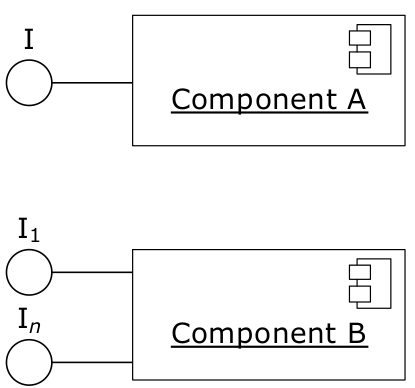
\includegraphics[width=0.5\textwidth]{figures/multipleinterfaces.png}
\caption{One or multiple interfaces}
\end{figure}

\hypertarget{stateless-versus-stateful}{%
\subsubsection{Stateless versus
Stateful}\label{stateless-versus-stateful}}
A stateful Object contains Properties which you can normaly set or get. Wheares a stateless object turns parameter input to a certain output.
\begin{lstlisting}
// Stateless
interface Calculator {
    double add(double a, double b);
    double subtract(double a, double b);
    double multiply(double a, double b);
    double divide(double a, double b);
}

// Stateful
interface Calculator {
    // add, subtract, ... as above
    void memoryAdd(double x);
    void memorySubtract(double x);
    double memoryRead();
    void memoryClear();
}
\end{lstlisting}


\hypertarget{minimal-versus-complete}{%
\subsubsection{Minimal versus Complete}\label{minimal-versus-complete}}

\begin{itemize}
\tightlist
\item
  Minimal interface

  \begin{itemize}
  \tightlist
  \item
    Has just the methods that a caller needs
  \end{itemize}
\item
  A more complete interface

  \begin{itemize}
  \tightlist
  \item
    Add additional methods (for convenience or efficiency)
  \end{itemize}
\item
  Alternative: Create another interface, and let the components choose
  to implement the basic one or both
\end{itemize}

\hypertarget{polymorphism-with-inheritance-versus-polymorphism-with-interfaces}{%
\subsection{Polymorphism with Inheritance versus Polymorphism with
Interfaces}\label{polymorphism-with-inheritance-versus-polymorphism-with-interfaces}}

Polymorphism describeds that you can change the behavior of things
(probably objetcs) during the runtime.

\begin{itemize}
\tightlist
\item
  An abstract base class probably already implements some methods or
  logic

  \begin{itemize}
  \tightlist
  \item
    This creates higher dependencies
  \end{itemize}
\item
  An interface does not implement any logic at all
\item
  You are able to extend from multiple interfaces but only from one
  superclass
\end{itemize}

\hypertarget{comparison}{%
\subsubsection{Comparison}\label{comparison}}

\begin{itemize}
\tightlist
\item
  Using inheritance

  \begin{itemize}
  \tightlist
  \item
    Advantage -- less delegation of common operations
  \end{itemize}
\item
  Using interfaces:

  \begin{itemize}
  \tightlist
  \item
    Advantage -- delay forming class hierarchy until usage is known
  \end{itemize}
\end{itemize}

\hypertarget{remote-interfaces}{%
\subsection{Remote Interfaces}\label{remote-interfaces}}

\hypertarget{procedural-style}{%
\subsubsection{Procedural style}\label{procedural-style}}

\begin{itemize}
\tightlist
\item
  look like local calls (= RPC style)
\item
  code must handle communication failures
\item
  typical request/response (synchronous) interactive usage
    \subitem 
  \textbf{Advantages :} Remote and local interfaces can appear the same.
  \subitem 
  \textbf{Disadvantages :} Can require more communication.
\end{itemize}

\hypertarget{document-style}{%
\subsubsection{Document style}\label{document-style}}

\begin{itemize}
\tightlist
\item
  replaces a series of calls with one call (and possible answer)
\item
  parameters and response values are encapsulated in send/receive
  messages (as ``documents'')
  
  \subitem 
  \textbf{Advantages :} Encapsules all required data from a service in one call.
  \subitem 
  \textbf{Disadvantages :} We have to process document further to get parameters.
\end{itemize}

\hypertarget{synchronous---asynchronous}{%
\subsubsection{Synchronous -
asynchronous}\label{synchronous---asynchronous}}

\begin{itemize}
\tightlist
\item
  Synchronous

  \begin{itemize}
  \tightlist
  \item
    Advantages

    \begin{itemize}
    \tightlist
    \item
      Practically immediate response
    \end{itemize}
  \item
    Disadvantages

    \begin{itemize}
    \tightlist
    \item
      Caller remains blocked till response arrives
    \item
      Does not scale well
    \end{itemize}
  \end{itemize}
\item
  Asynchronous

  \begin{itemize}
  \tightlist
  \item
    Advantage

    \begin{itemize}
    \tightlist
    \item
      Scales well
    \end{itemize}
  \item
    Disadvantage

    \begin{itemize}
    \tightlist
    \item
      Where should documents (parameters) be validated?
    \end{itemize}
  \end{itemize}
\end{itemize}

\hypertarget{stateless-stateful}{%
\subsubsection{Stateless -- stateful}\label{stateless-stateful}}

\begin{itemize}
\tightlist
\item
  Stateless

  \begin{itemize}
  \tightlist
  \item
    Advantages

    \begin{itemize}
    \tightlist
    \item
      Servers scale easily: any server can handle request
    \item
      Service has redundancy: any server could go down and the client
      could continue with another server
    \end{itemize}
  \item
    Disadvantages

    \begin{itemize}
    \tightlist
    \item
      Amount of state information that must be passed back and forth
      between client and server.
    \end{itemize}
  \end{itemize}
\item
  Stateful

  \begin{itemize}
  \tightlist
  \item
    Advantages

    \begin{itemize}
    \tightlist
    \item
      Server maintains conversional state per client
    \item
      Less data communication between client and server
    \end{itemize}
  \item
    Disadvantages

    \begin{itemize}
    \tightlist
    \item
      State recovery in case of server crash
    \item
      Scalability
    \end{itemize}
  \end{itemize}
\end{itemize}

\hypertarget{rest}{%
\subsubsection{REST}\label{rest}}
A RESTful API is an application program interface (API) that uses HTTP requests to GET,PUT, POST and DELETE data.
\begin{itemize}
\tightlist
\item
  Client/Server
\item
  Stateless
\item
  Cachable
\item
  WebService APIs offering REST over HTTP
\item
  Consists of

  \begin{itemize}
  \tightlist
  \item
    Base URL
  \item
    Internet media type
  \item
    Standard HTTP methods
  \item
    Hypertext links to represent the state
  \item
    Links to other resources
  \end{itemize}
\end{itemize}

\hypertarget{methods}{%
\paragraph{Methods}\label{methods}}

\begin{itemize}
\tightlist
\item
  Safe Methods:

  \begin{itemize}
  \tightlist
  \item
    No changes on the data
  \item
    i.e.~only read operations
  \end{itemize}
\item
  Idempotent Operations:

  \begin{itemize}
  \tightlist
  \item
    Multiple executions of the operations does not change the data
  \end{itemize}
\end{itemize}

\begin{figure}[H]
\centering
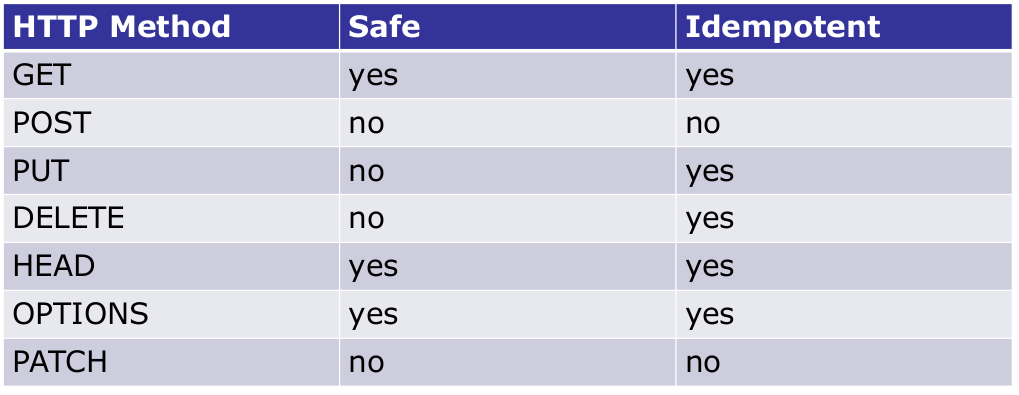
\includegraphics[width=0.5\textwidth]{figures/httpMethods.png}
\caption{HTTP Methods}
\end{figure}


\begin{figure}[H]
\centering
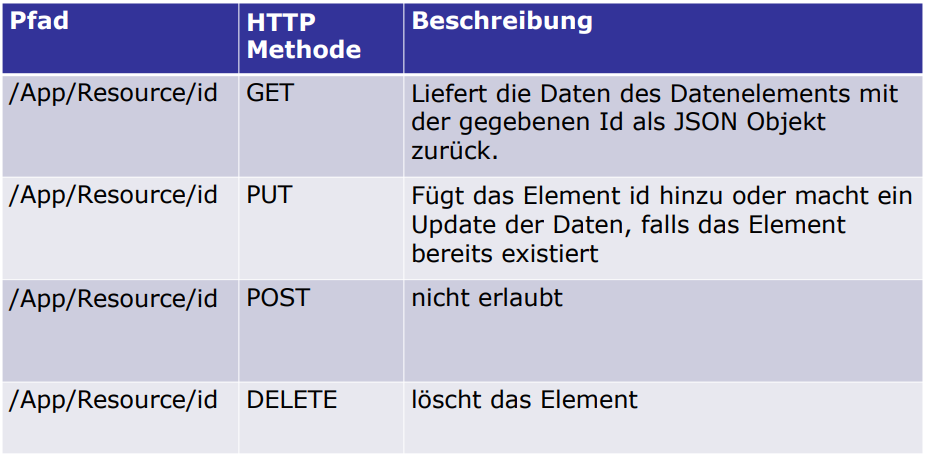
\includegraphics[width=0.5\textwidth]{figures/RestCAlls.PNG}
\caption{Calls With REST}
\end{figure}

\hypertarget{coupling-and-cohesion}{%
\subsection{Coupling and Cohesion}\label{coupling-and-cohesion}}

\begin{itemize}
\tightlist
\item
  Good Design $ \approx $ Low Coupling \& High Cohesion

  \begin{itemize}
  \tightlist
  \item
    old principles, but often forgotten
  \item
    can be really hard to get right!
  \item
    see also Parnas' paper ``On the Criteria To Be Used in Decomposing
    Systems into Modules''
  \end{itemize}
\end{itemize}


\hypertarget{good-interface-design}{%
\subsection{Good (Interface) Design}\label{good-interface-design}}




\begin{itemize}
\tightlist
\item
  Separate Query and Action

  \begin{itemize}
  \tightlist
  \item
    either obtain state or change state of a component
  \end{itemize}
\item
  Three Laws of Interfaces (Ken Pugh)

  \begin{itemize}
  \tightlist
  \item
    An interface shall do what its methods say it does
  \item
    An interface shall do no harm
  \item
    If an implementation is unable to perform its responsibilities, it
    shall notify its caller
  \end{itemize}
\item
  Manage Dependencies! (Robert Martin)

  \begin{itemize}
  \tightlist
  \item
    SOLID principles
  \end{itemize}
\end{itemize}

\hypertarget{solid}{%
\subsubsection{SOLID}\label{solid}}

\begin{itemize}
\tightlist
\item
  Single Responsibility Principle

  \begin{itemize}
  \tightlist
  \item
    high cohesion, only one reason to change
  \end{itemize}
\end{itemize}

\begin{figure}[H]
\centering
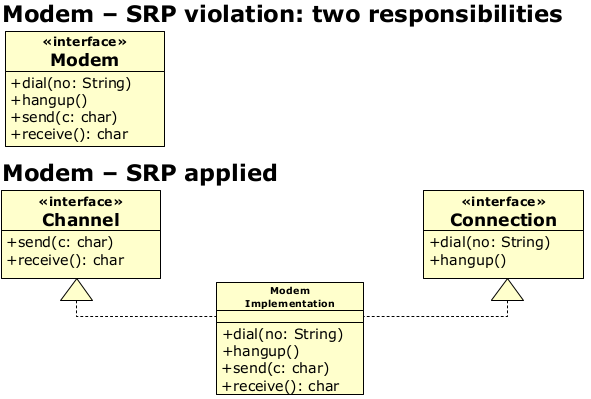
\includegraphics[width=0.5\textwidth]{figures/singleresponsibility.png}
\caption{Single Responsibility Example}
\end{figure}


\begin{itemize}
\tightlist
\item
  Open - Closed Principle

  \begin{itemize}
  \tightlist
  \item
    open for extension, closed for change
  \end{itemize}
\end{itemize}

\begin{figure}[H]
\centering
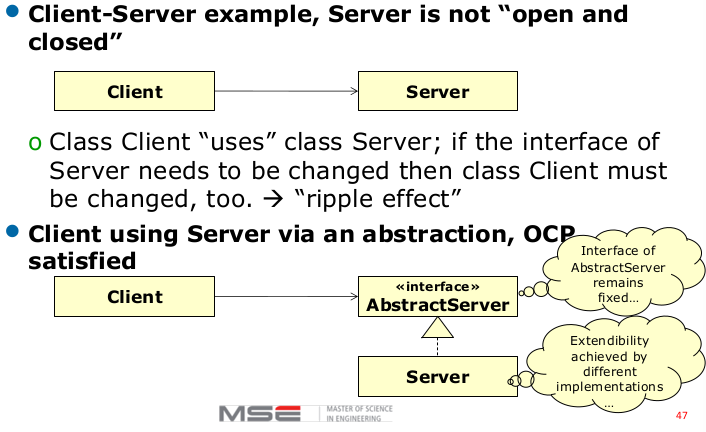
\includegraphics[width=0.5\textwidth]{figures/open-closedprinciple.png}
\caption{Open-Closed Example}
\end{figure}

\begin{itemize}
\tightlist
\item
  Liskov Substitution Principle

  \begin{itemize}
  \tightlist
  \item
    subclasses fulfill superclasses'/interface's role
  \item
    In the following example, the square implementation doesn't fulfill
    the setSides() method of the rectangle properly.
  \end{itemize}
\end{itemize}

\begin{figure}[H]
\centering
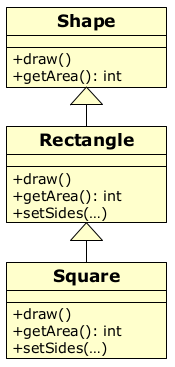
\includegraphics[width=0.2\textwidth]{figures/lspexample.png}
\caption{Liskov Substitution Example}
\end{figure}


\begin{itemize}
\tightlist
\item
  Interface Segregation Principle
\begin{figure}[H]
\centering
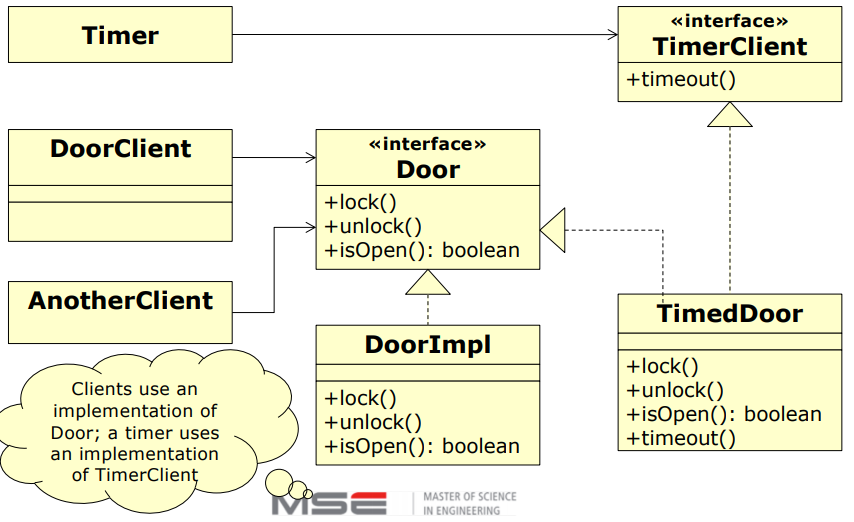
\includegraphics[width=0.5\textwidth]{figures/InterfaceSegregationPrinciple.PNG}
\caption{Interface Segregation Principle}
\end{figure}

  \begin{itemize}
  \tightlist
  \item
    split ``fat'' interfaces to gain higher cohesion
  \item
    clients should not be forced to depend on interface features they do
    not use
  \end{itemize}
\item
  Dependency Inversion Principle

  \begin{itemize}
  \tightlist
  \item
    high-level classes should not depend upon low-level classes; both
    should depend on abstraction
  \item
    abstractions should not depend on details; details should depend on
    abstractions
  \end{itemize}
\end{itemize}

\begin{figure}[H]
\centering
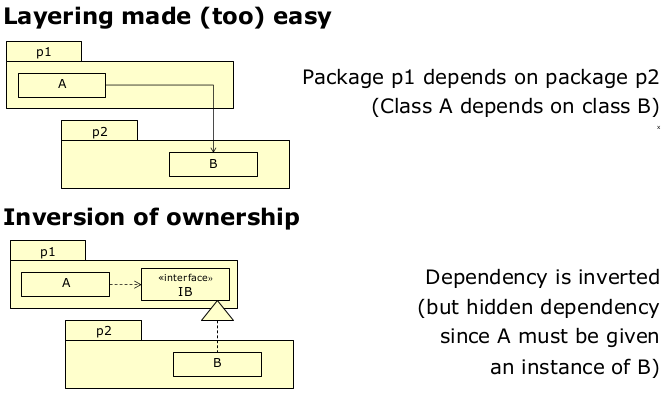
\includegraphics[width=0.5\textwidth]{figures/dipexample.png}
\caption{Dependency Inversion Example}
\end{figure}

\clearpage